\documentclass[]{article}
%opening
\title{Writeup Document}
\author{Alex Miller}
\addtolength{\oddsidemargin}{-.875in}
\addtolength{\evensidemargin}{-.875in}
\addtolength{\textwidth}{1.75in}

\addtolength{\topmargin}{-.875in}
\addtolength{\textheight}{1.75in}
\setcounter{secnumdepth}{0}
\usepackage{cancel}
\usepackage{amssymb}
\usepackage{amsmath}
\usepackage{hyperref}
\usepackage{graphicx}
\graphicspath{ {./} }
\usepackage[ruled,vlined, linesnumbered]{algorithm2e}
\DontPrintSemicolon


\begin{document}
	\maketitle

\section{Changes}
	\subsection{Changes to the design}
	My final design ended up including three distinct modules as opposed to the previously proposed two; these included a graph generation module (graph.py), a Floyd-Warshall module (graph.c, floyd.c), as well as a testing module (fw\_serial.c, fw\_parallel.c, test\_script.sh). Describing these pieces in the order in which they are salient:
	\begin{itemize}
		\item graph.py describes a simple python script that randomly generates an adjacency matrix of specified length and stores it in an appropriately named text file. These files are used to test the performance of the functions described in floyd.c. I added this module in order to cut down on the time that I would need to spend making example graphs. 
		
		It is notable that the adjacency matrix produced by this script don't include negative edge weights. This is on purpose; the presence of negative edges would require me to test input matrices for negative cycles, as Floyd-Warshall only works for graphs without such cycles. I also don't think that the presence of negative edge weights should impact the performance of a Floyd-Warshall implementation, regardless of whether it is parallelized or not. Therefore, rather than choosing to include possibly negative edge weights in my input matrices and having to go through the extra difficulty of testing my randomly generated inputs, I chose to not include negative edges alltogether.
		
		\item floyd.c describes serial and parallelized implementations of Floyd-Warshall. We will discuss the changes to this module later. For now just keep in mind that the serial implementation is called fw\_serial and the parallel implementation fw\_parallel. graph.c still describes the I/O methods by which preliminary adjacency matrices are loaded into memory as a graph\_t instance and results are written to text files.
		\item fw\_serial.c describes a simple program that loads an adjacency matrix from a text file, performs an operation of fw\_serial, and writes the result to a text file. The name of this text file is formatted like a row of a csv file; it has the form $res/<n>,<t>,<time>$ where:
		\begin{itemize}
			\item $<n>$: An integer describing how many vertices were in the graph used to generate the result
			\item $<t>$: An integer describing how many threads were used in computing the result. For all operations of fw\_serial this value is 1. For operations of fw\_parallel it may be 1, 2, 4, 8, 18, 32, or 64
			\item $<time>$: A float representing how many miliseconds it takes to generate a result. This measurement reflects the time it takes for the methods fw\_serial() or fw\_parallel() (as described in hw1/floyd.c) to return.
		\end{itemize}	
		fw\_parallel.c is similar, but utilizes fw\_parallel (using a specified number of threads) instead. 
		\\
		test\_script.sh performs all necessary testing by running the following:
		\begin{itemize}
			\item For $n \in$ [16, 32, 64, 128, 256, 512, 1024]:
			\begin{itemize}
				\item ./fw\_parallel n.txt 1
				\item ./fw\_serial n.txt 1
				\item For $t \in$ [2, 4, 8, 16, 32, 64]:
				\begin{itemize}
					\item ./fw\_parallel n.txt t
				\end{itemize}
			\end{itemize}
		\end{itemize}
		It takes the results of those tests and arranges them accordingly:
		\begin{itemize}
			\item Results from './fw\_serial n.txt 1' are left in the $hw1/res/$ folder, unchanged. The contents of these files are used to verify results of ./fw\_parallel
			\item Results from './fw\_parallel n.txt 1' are placed in the $hw1/exp1$ folder. Their names are changed to include the run-times of results from './fw\_serial n.txt'. We will discuss how this is done later.
			\item Results from $./fw\_parallel n.txt t$ are placed in the 'hw1/exp1/t' folder. Their names are changed to include the run-times of results from './fw\_serial n.txt'.  We will discuss how this is done later.
		\end{itemize}
		The purpose of this is to make it easy to generate .csv files containing the relevant data for both experiment 1 and 2. These files are compiled and saved in the $hw1/exp\_data$ folder

		I chose to make this change to my testing structure because my original design tested fw\_serial and fw\_parallel in the same file, which I thought would account for unnecessarily long testing periods; there is no need to retest my serial version every time I want to test my parallel version. Using a bash script also made it easy to test these two different executables separately while also keeping track of and organizing result data. Furthermore, putting everything in a bash file made testing easy to do with slurm.The basic logic of my test plan did not change; I verified correctness of each module before moving on the next and checked the results of fw\_parallel using those of fw\_serial
	\end{itemize}
	As per the specific modifications I made to my design of floyd.c: My conception of fw\_serial remained unchanged throughout this process. However, my design for fw\_parallel changed a lot. Our discussion last Tuesday made me realize that by statically partitioning the matrix into equal sized blocks, I could utilize all the threads that I am given access to in a given experiment, rather than being bounded by the number of vertices in a given graph. More correctly, I should say that the new bound of how many threads can be employed for a given graph is the number of indices in its adjacency matrix (the number of vertices squared) rather than the number of vertices in the graph. However, this increase in our ability to utilize thread brought certain drawbacks: 
	\begin{itemize}
		\item Since such blocks aren't guaranteed to be squares, this method would require more overhead in generating the geometry of the partitioning of the matrix. However, the dimensions themselves could be stored in the graph\_t data type I designed before, allowing all threads to know the area of the blocks they are being asked to compute.
		\\
		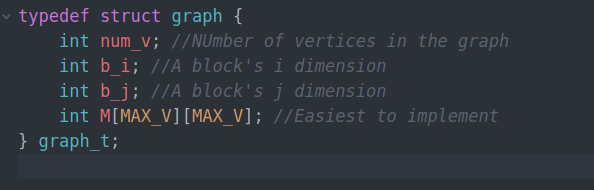
\includegraphics[scale=0.5]{code/graph_t.png}
		\item Threads would have to know one more piece of information in order to operate; instead of just needing to know what row index they were working on, they would need to know the corner indices from which to begin computing their assigned blocks. 
		\item Furthermore, If I wanted to synchronize the operation of these threads I would need to pass them all a pointer to a thread barrier
	\end{itemize}
	However, by allowing for the use of more threads, it was my thought that I could increase performance, at the very least for larger adjacency matrices where the larger amount of overhead of managing many threads would pay off in improved run times.
	\\\\
	I maintain the same invariants as before; threads still wait for a the matrix to be computed for a given value of $k$ before computing the matrix for $k + 1$; moreover, the block structure still reflects the independence of the order in which indices are computed. As stated in my previous design document: As an invariant, we know that we will always have generated the shortest path lengths of all $(i,j)$ pairs for a value of $k$ before we generate such lengths for a value of $k + 1$, maintaining data dependencies within the algorithm.
	\subsection{Changes in hypotheses}
	I did not implement my past design before attempting my current, so I cannot speak to improvements in performance of one in relation to the other. I maintain, in general, same hypotheses as I did before, with the following caveats:
	\begin{itemize}
		\item I do not expect to see similar cache performance between my serial and parallel implementations of Floyd-Warshall; considering that we are reading my blocks as opposed to rows, there is no reason to think that fw\_serial's cache will look like that of fw\_parallel
		\item I expect to see minimal speedup, or even slowdown for small graphs with few vertices; the increased overhead of using as many threads as possible should detract from any gains in performance for sufficiently small input spaces. However, we may see gains in performance for graphs with 16, 32, or 64 vertices
		\item For large enough graphs, I expect to see speedup that is linear in proportion to the amount of threads used, and not bounded by the number of threads that can be used at any one time.
	\end{itemize}
\section{Results}
	The performance data for experiments 1 and 2 is stored in a folder called $hw1/exp\_data$. This folder contains the .csv files that describe performance data for a given experiment. More specifically, they describe how fw\_serial compares to fw\_parallel in terms of run time. The columns of these files are:
	\begin{itemize}
		\item Number of vertices : How many vertices did the graph for which a result was computed contain?
		\item Number of threads : How many threads were used by fw\_parallel to compute this result?
		\item Run-time : How long did it take fw\_parallel to generate this result
		\item Serial Time : How long did it take fw\_serial to generate the same result for the same graph?
	\end{itemize}
	I took this data and plotted it using Google sheets. This file can be found \href{https://docs.google.com/spreadsheets/d/1XrjW1c_qoefwkYxm_nAwCrnQ4Z4TFlYyeFtUYgdvXZE/edit?usp=sharing}{here}. A copy of this data is also available in a .pdf that can be located at $hw1/hw1\_result\_data.pdf$. The following graphs represent this data as well.
	
	\subsection{Exp 1 Data Visuals}
		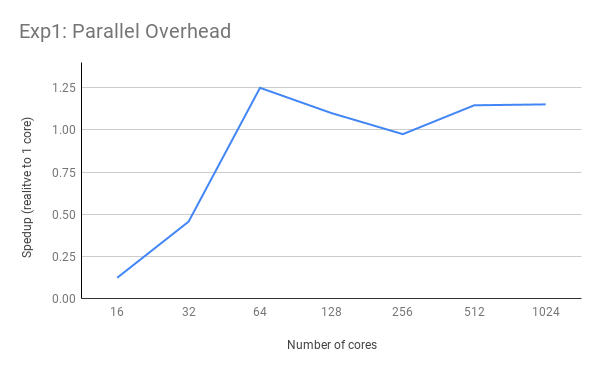
\includegraphics[scale=0.5]{graphs/exp1.png}
	
	\subsection{Exp 2 Data Visuals}
	
		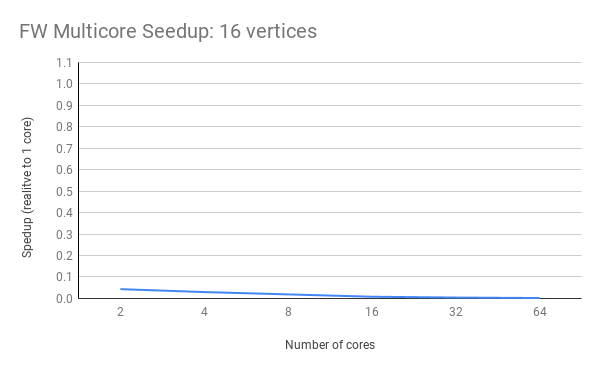
\includegraphics[scale=0.5]{graphs/exp2_16.png}\\
		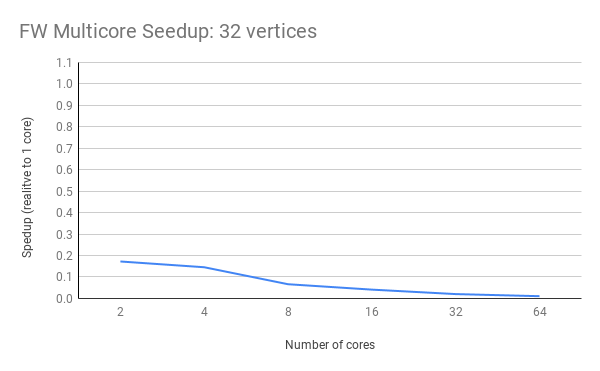
\includegraphics[scale=0.5]{graphs/exp2_32.png}\\
		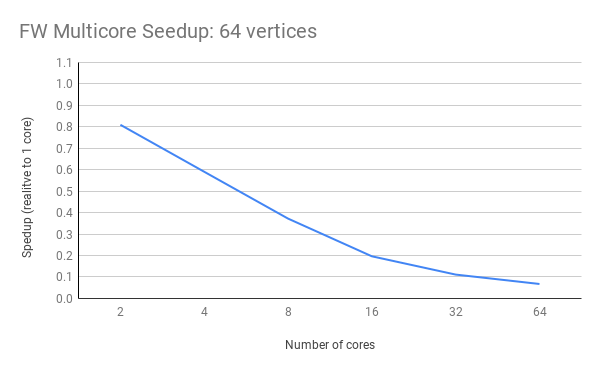
\includegraphics[scale=0.5]{graphs/exp2_64.png}\\
		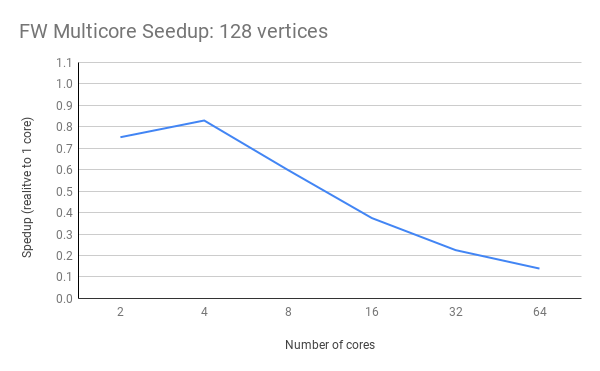
\includegraphics[scale=0.5]{graphs/exp2_128.png}\\
		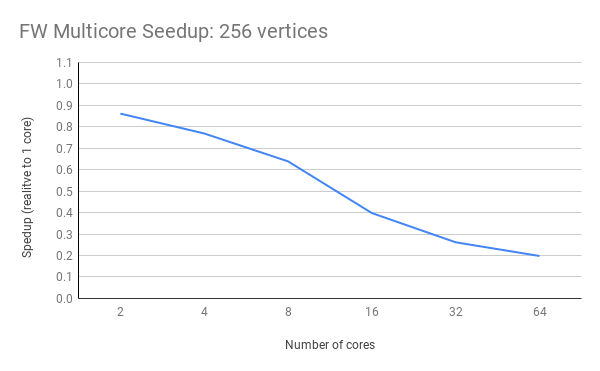
\includegraphics[scale=0.5]{graphs/exp2_256.png}\\
		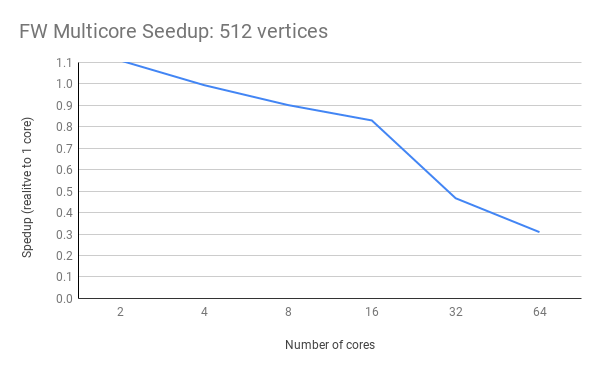
\includegraphics[scale=0.5]{graphs/exp2_512.png}\\
		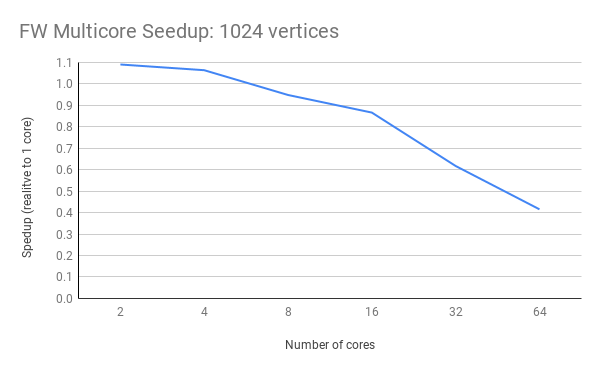
\includegraphics[scale=0.5]{graphs/exp2_1024.png}\\

\section{Analysis}
	\subsection{Exp1}
	
	 
	As the data demonstrates, fw\_parallel suffered significant slowdown in relation to fw\_serial for sufficiently small input spaces, namely graphs containing 16 and 32 vertices. However, for larger input spaces, fw\_parallel suffered little slowdown, and even speedup for some input spaces. This result is perplexing; why, after all, should fw\_parallel outperform fw\_serial while only utilizing only one additional core, given its additional overhead in computing an appropriate block size (the whole matrix, in this case) and launching a seperate thread to compute a result? This perhaps can be explained by the fact that such overhead is minimal in comparison to the work required to run a serial implementation of Floyd-Warshall on such a large input space. However, this still wouldn't explain why we should observe speedup. Alternatively, or perhaps, complimentary, such a result may also be explained by run time aberrations on the CS department's slurm system which could slightly augment the speeds at which fw\_parallel and fw\_serial return. This could explain why we observe speedup. In future studies, I would increase the number of trials used to collect this data; I only used one, but perhaps if I did nine more I would have smoother data, without the presence of such speedups.
	\\\\
	To some extent, these data do confirm my hypothesis, which I will repeat:
	\\
	\textit{"I expect to see minimal speedup, or even slowdown for small graphs with few vertices; the increased overhead of using as many threads as possible should detract from any gains in performance for sufficiently small input spaces. However, we may see gains in performance for graphs with 16, 32, or 64 vertices"}
	\\
	As I expected, overhead, at least in experiment 1, became a negligible factor for "sufficiently" large input space. However, it is important to keep in mind that the way fw\_parallel is declared, its overhead increases with the number of threads specified by the user. For example, consider the following section of $fw\_parallel()$ as declared in $hw1/floyd.c$:
	\\
			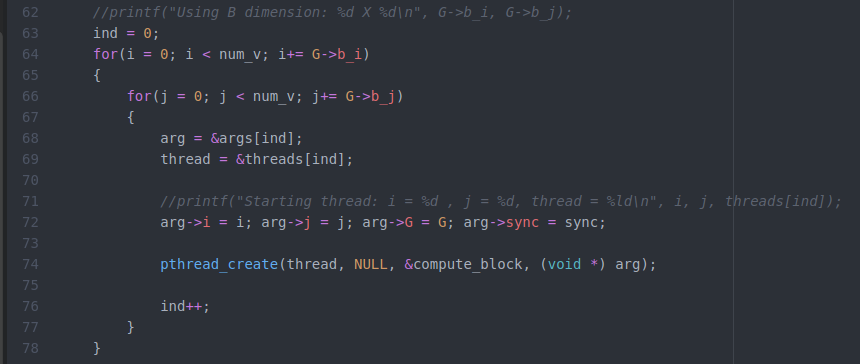
\includegraphics[scale=0.5]{code/ex1.png}
	\\
	Within this section, pthread\_create is invoked $t$ times, where $t$ is the number of threads specified by a user. This can create significant overhead for sufficiently large values of $t$, but we wouldn't notice this overhead for smaller values of $t$, such as $t = 1$.
	\\\\
	Therefore, while we observe minimal impacts on fw\_parallel's run-time (while using only one additional thread) due to overhead for sufficiently large input spaces, we should not necessarily expect that same observation in experiment 2, where fw\_parallel's run-time is put to the test while using multiple threads. This should impose a limit on the amount of speedup we can expect in experiment 2.
	
	\subsection{Exp2}
	As the data shows, my parallel implementation of Floyd-Warshall failed to deliver noticeable improvement over my serial implementation when using multiple threads. If anything, the extra overhead of parallelizing Floyd-Warshall with many threads seemed to heavily outweigh any potential benefit from having multiple concurrent processes computing results for distinct blocks of vertices.
	\\\\
	That being said, it is notable that for larger graphs with more vertices, my implementation of fw\_parallel did deliver slight speedup. However, this observed speedup did not confirm my hypothesis that for larger graphs, speedup would appear linearly proportional to the number of threads utilized. Rather, for the trials testing performance on graphs containing 512 and 1024 vertices, maximum possible speedup (given my implementation) was achieved using 2 or 4 threads, with drop offs in performances being observed for larger thread counts. This can be explained by increased overhead in the creation and maintenance of greater numbers of threads, which could be detracting from any speedup due to increased parallelization.
	\\\\
	Overall, I seem supported in my hypothesis that observed speedup would increase with the size of the input space. However, it also seems that I require a new model by which to predict speedup since I did not observe linear speedup. This lack of support for my hypothesis indicates to me that the overhead of managing and utilizing as many threads as possible does not pay off in increased performance necessarily. I do wonder, however, whether or not I would observe something closer to linear speedup if I were to test a large enough input space; though I did not observe linear speedup, the curves of my data display a tendency to flatten for larger input spaces. Perhaps I might observe something close to linear speedup proportional to the number of threads used for large enough graphs.
	\\

\section{Theory Questions}
Provide solutions to questions 2, 3, 4, 5, 7, 8, 11, 14, 15, 16.

\subsection{Problem 2}
\begin{enumerate}
	\item Liveliness; the good thing that eventually happens is that all patrons will be served
	\item Safety; the bad thing that never happens is that things float away into the air
	\item Safety; the bad thing that never happens is that the program gets stuck
	\item Liveliness; the good thing that eventually happens is that the user is informed of the event
	\item Liveliness; the good thing that eventually happens is that the user is informed of the event
	\item Safety; the bad thing that never happens is that the cost of living decreases
	\item Liveliness; the good thing that eventually happens is that I will die and have to pay taxes 
	\item Safety; the bad thing that never happens is that I never get snuck up on by a Harvard man.
\end{enumerate}
\subsection{Problem 3}
Alice and Bob set cans up on each other's window sills; each one's can has a string attached to it that the other can use to knock it down.
Alice does the following:
\begin{enumerate}
	\item She waits until the can on her window sill is down.
	\item She releases the pets.
	\item When the pets return, Alice checks whether they finished the food. If so, she resets the can on her windowsill and then knocks down the can on Bob's window sill.
\end{enumerate}
Bob does the following:
\begin{enumerate}
	\item He waits until the can on his window sill is down.
	\item He puts food in the yard.
	\item He resets the can on his window sill and knocks down the can on Alice's window sill.
\end{enumerate}
\subsection{Problem 4}
The following assume $P \geq 2$
In the case that we know the initial state of the switch is off:
\begin{itemize}
	\item We designate one of the $P$ prisoners to be the $counter$; the counter maintains an internal count $c$. Initially, $c = 0$.
	\item When the counter enters the switch room:
	\begin{itemize}
		\item If the switch is down, they do nothing and leave
		\item If the switch is up, the counter increments $c$
	\end{itemize}
	\item When $c = P - 1$, the counter may declare that all $P$ prisoners have visited the switch room at least once
	\item For all other prisoners; when they enter the switch room:
	\begin{itemize}
		\item If the switch is down, and they have never flipped the switch before, they should switch it to the "on" position. Otherwise, they should do nothing and leave.
		\item If the switch is up, they should do nothing and leave.
	\end{itemize}
\end{itemize}
In the case that we don't know the initial state of the switch:
\begin{itemize}
	\item We designate one of the $P$ prisoners to be the $counter$; the counter maintains an internal count $c$. Initially, $c = 0$.
	\item When the counter enters the switch room:
	\begin{itemize}
		\item If the switch is down, they do nothing and leave
		\item If the switch is up, the counter increments $c$
	\end{itemize}
	\item When $c = (2 * P) - 1$, the counter may declare that all $P$ prisoners have visited the switch room at least once
	\item For all other prisoners; when they enter the switch room:
	\begin{itemize}
		\item If the switch is down, and they have not flipped the switch more than once, they should switch it to the "on" position. Otherwise, they should do nothing and leave.
		\item If the switch is up, they should do nothing and leave.
	\end{itemize}
\end{itemize}
\subsection{Problem 5}
Starting from the back of the line, the first prisoner does the following:
\begin{itemize}
	\item If they see an odd number of red hats in front of them, they call out "red!"
	\item Otherwise, they call out "blue!"
\end{itemize}
The next prisoner does the following:
\begin{itemize}
	\item If the previous prisoner called out "red!":
	\begin{itemize}
		\item If there are an odd number of red hats in front of them, they know they must not be wearing a red hat. They should call out "blue"
		\item Otherwise, they know they are wearing a red hat. They should call out "red"
	\end{itemize}
	\item If the previous prisoner called out "blue!":
	\begin{itemize}
		\item If there are an odd number of red hats in front of them, they know they must be wearing a red hat. They should call out "red"
		\item Otherwise, they know they are wearing a blue hat. They should call out "blue"
	\end{itemize}
\end{itemize}
Likewise, every prisoner following the first can know what hat they are wearing by:
\begin{enumerate}
	\item Knowing whether or not there were initially an even number of red hats or not by remembering the first prisoner's answer
	\item Counting how many red and blue hats were claimed by each prisoner after the first
	\item Deducing the color of their hat from how many red and blue hats have been claimed (excluding the first prisoner), the initial eveness in the number of red hats, as well as the evenness in the number of red and blue hats in front of them.
\end{enumerate}
\subsection{Problem 7}
$S_n = \frac{1}{1 - p + \frac{p}{n}}$ \\
$S_2 = \frac{1}{1 - p + \frac{p}{2}}$ \\
$S_2 = \frac{1}{1 - \frac{p}{2}}$ \\
$1 - \frac{p}{2} = \frac{1}{S_2}$ \\
$p = 2 - \frac{2}{S_2}$ \\
$S_n = \frac{1}{1 - (2 - \frac{2}{S_2}) + \frac{(2 - \frac{2}{S_2})}{n}}$\\

\subsection{Problem 8}
\begin{itemize}
	\item Let $proc-a$ denote a uni-processor that executes five instructions per second
	\item Let $proc-b$ denote a ten processor multi-processor, each core of which executes 1 instruction per second
	\item Let $P$ be a program we are considering to run on either $proc-a$ or $proc-b$. The fraction of $P$ that is parallelizable is $p$.
	\item Let $A$ be the time it takes for $proc-a$ to run $P$
	\item Let $B_i, 0 \leq i \leq 10$ be the time it takes for $proc-b$ to run $P$ using $i$ cores
	\item $5 * A = B_1$
	\item $B_{10} = \frac{1}{1 - p + \frac{p}{10}} = \frac{1}{1 - \frac{9p}{10}}$
	\item Assume that $P$ runs faster on $proc-b$ than $proc-a$ while using all ten cores:
	\begin{itemize}
		\item That must mean that $B_{10}$ achieves a speedup ratio of $5$ or more in relation to $B_1$
		\item Therefore $B_{10} \geq 5$
		\item $\frac{1}{1 - \frac{9p}{10}} \geq 5$
		\item $\frac{9p}{10} \geq 1 - \frac{1}{5}$
		\item $\frac{9p}{10} \geq \frac{4}{5}$
		\item $9p \geq 8$
		\item $p \geq \frac{8}{9}$
	\end{itemize}
	\item Therefore, if $P$ runs better on $proc-b$ than $proc-a$, it must be that  $p \geq \frac{8}{9}$. 
	\item Therefore, if $p > \frac{8}{9}$, we should buy $proc-b$, and $proc-a$ if otherwise.
\end{itemize}

\subsection{Problem 11}
The protocol satisfies mutual exclusion:
\begin{itemize}
	\item Assume that it does not and consider the steps of two threads, $A$ and $B$
	\item Therefore the following relationships must hold:
	\begin{enumerate}
		\item $write_A(turn = A) \rightarrow write_B(turn = B) \rightarrow CS_A$
		\item $write_B(turn = B) \rightarrow write_A(turn = A) \rightarrow CS_B$
	\end{enumerate}
	\item Consider these relationships assuming a specified ordering by which the threads enter the critical section. WLOG,  that $B$ is the last thread to write a value to $turn$ before entering the critical section; therefore
	\begin{enumerate}
		\item $write_A(turn = A) \rightarrow write_B(turn = B)$
	\end{enumerate}
	If the lock is not mutually exclusive, as we assume it is, this means that $B$ must enter it's critical section before $A$ leaves its. However, $B$ cannot enter its critical section until $A$ leaves its critical section and $write_A(turn = A)$. Therefore $B$ waits for $A$ to leave the $CS_A$ before it enters $CS_B$. Therefore for some $i, j, CS_A^i \rightarrow CS_B^j$
	\item By contradiction, the lock is mutually exclusive.
\end{itemize}
The protocol is not deadlock free. Consider the following execution:
\\
	$write_A(turn = A) \rightarrow read_A(busy == false) \rightarrow write_A(busy = true)\rightarrow write_B(turn = B)$
\\
After this point, $busy$ never stops being true, so $B$ never stops setting $turn$ to $B$, so $A$ never exits its outer loop and never enters its critical section.
\\
Because the protocol suffers from deadlock, it also suffers from starvation.
\subsection{Problem 14}
Assuming that $n > \l$, we can get the desired behavior out of the existing filter lock design by reducing that sizes of the $level$ and $victim$ arrays from $n$ to $n - (\l - a)$ and reflecting that change in our loop structure so as not not iterate outside the bounds of our (now smaller) data structures. This should be enough.
\subsection{Problem 15}
The scientists are wrong in their claim.
\begin{enumerate}
	\item Consider the execution of two threads, $A$ and $B$, acquiring the FastPath lock at the same time:
	\begin{itemize}
		\item $write_A(x = A) \rightarrow read_A(y == -1) \rightarrow write_A(y = A) \rightarrow read_A(x == B)$
		\item $write_B(x = B) \rightarrow read_B(y == -1) \rightarrow write_B(y = B) \rightarrow read_B(x == A)$
	\end{itemize}
	\item WLOG, assume that $B$ acquires the lock shortly after $A$ and that $write_A(x = A) \rightarrow write_B(x = B)$
	\item Assuming that $y = -1$ initially, it can happen that $A$ and $B$ both read $y == -1$ before either have the chance to $write_{A or B}(y = A or B)$
	\item Therefore it is possible for neither thread to wait in the while loop in line 8 of the declaration of FastPath.
	\item Because $write_A(x = A) \rightarrow write_B(x = B)$, $write_A(x = A) \rightarrow write_B(x = B) \rightarrow read_A(x == B)$; $A$ can proceed to call the base lock(). But because $write_B(x = B) \rightarrow read_B(x == B)$, $B$ never calls the base lock(); instead it just proceeds to $CS_B$.
	\item Therefore both threads can enter the Critical Section at the same time, because one does not even need to call the base lock in order to proceed past the FastPath wrapper lock. This violates any mutually exclusive property the base Lock may have.
	\item Therefore it is not the case that our scientists' FastPath wrapper is mutually exclusive and starvation free $\Leftrightarrow$ the base Lock is.
\end{enumerate}
\subsection{Problem 16}
At most one thread gets the value STOP:
\begin{itemize}
	\item Consider two threads, $A$ and $B$
	\item Assume that $A$ returned STOP
	\item Therefore the ordering $write_A(last = A) \rightarrow read_A(goRight == False)\rightarrow write_A(goRight = True) \rightarrow read_A(last == A)$ occurs
	\item Assume that $B$ also returns STOP, but after $A$
	\item If this is the case then $read_A(last == A) \rightarrow write_B(last = B) \rightarrow read_B(goRight == False) \rightarrow write_B(goRight = True) \rightarrow read_B(last == B)$
	\item However, $read_B(goRight == False)$ never occurs because $goRight$ is set to true by $A$ and is never set to false again anywhere in the program.
	\item Therefore $B$ would return RIGHT, and not STOP.
	\item WLOG, assume that thread $B$ is some thread that comes after some thread $A$ which returns STOP. It can't be the case that $B$ also returns STOP, so at most one thread does.
	\item \textbf{QED}
\end{itemize}
At most $n - 1$ threads get the value DOWN.
\begin{itemize}
	\item Consider two cases:
	\begin{enumerate}
		\item One or more of $n$ threads return RIGHT; the amount of threads that could return DOWN is therefore at most $n - 1$.
		\item No threads return RIGHT. If this is the case then $\forall i, j \in [n], read_i(goRight == false) \rightarrow write_j(goRight = true)$. This also implies that there was some thread $k$ for which $write_k(last = k)$ occurred after all other $n$ threads. Therefore, if no threads return RIGHT, such a thread $k$ will evaluate $read_k(last == k)$ as $true$, in which case it would return STOP. In this case, then, the amount of threads that could return DOWN is $n - 1$.
	\end{enumerate}
	\item In either case, at most $n - 1$ threads get the value DOWN
	\item \textbf{QED}
\end{itemize}
At most $n - 1$ threads get the value RIGHT.
\begin{itemize}
	\item FSOC, Assume that no thread returns STOP or DOWN
	\item Therefore $\forall i \in [n], read_i(goRight == true)$
	\item However, for this to be true, $\exists j \in [n], write_j(goRight = true)$
	\item Such a thread however would never return RIGHT, as $write_j(goRight = true)$ never precedes a thread returning RIGHT
	\item Therefore, for all threads to return RIGHT, some thread must return either STOP or DOWN
	\item This is a constradiction, therefore not every thread can return RIGHT
	\item Therefore, at most $n - 1$ threads get the value RIGHT
	\item \textbf{QED}
\end{itemize}
\end{document}
